%% ---------------------------------------------------------------------------
%% Single-blind Tool Demonstration submission draft (authors shown).
%% 'nonacm' gives the ACM sigconf layout without the copyright/rights block,
%% so the draft compiles cleanly with no placeholder metadata. For camera-ready:
%% remove 'nonacm', then add \acmConference / \setcopyright / \acmDOI as provided
%% by the proceedings chairs.
%% ---------------------------------------------------------------------------
\documentclass[sigconf,nonacm]{acmart}

\settopmatter{printacmref=false, printfolios=true}
\pagestyle{plain}

\usepackage{tikz}
\usetikzlibrary{arrows.meta, positioning, fit, backgrounds, calc, shapes.geometric}
\usepackage{pifont}
\usepackage{listings}
\usepackage{enumitem}
\usepackage{colortbl}
\usepackage{pgfplots}
\pgfplotsset{compat=1.18}

\newcommand{\cmark}{\textcolor{green!60!black}{\ding{51}}}
\newcommand{\xmark}{\textcolor{black!30}{\ding{55}}}
\newcommand{\pmark}{\textcolor{orange!85!black}{$\sim$}}
\newcommand{\tool}{\textsc{Query Analyzer}}
\newcommand{\code}[1]{\texttt{\small #1}}

\lstset{
  basicstyle=\ttfamily\scriptsize,
  breaklines=true,
  columns=fullflexible,
  keepspaces=true,
  frame=tb,
  framesep=3pt,
  aboveskip=4pt,
  belowskip=2pt,
  xleftmargin=2pt,
  showstringspaces=false,
  language=Java
}

%% --- CCS concepts ---
\begin{CCSXML}
<ccs2012>
<concept>
<concept_id>10011007.10011074.10011099.10011102</concept_id>
<concept_desc>Software and its engineering~Software performance</concept_desc>
<concept_significance>500</concept_significance>
</concept>
<concept>
<concept_id>10011007.10011074.10011092</concept_id>
<concept_desc>Software and its engineering~Software testing and debugging</concept_desc>
<concept_significance>300</concept_significance>
</concept>
<concept>
<concept_id>10002951.10002952</concept_id>
<concept_desc>Information systems~Data management systems</concept_desc>
<concept_significance>300</concept_significance>
</concept>
</ccs2012>
\end{CCSXML}
\ccsdesc[500]{Software and its engineering~Software performance}
\ccsdesc[300]{Software and its engineering~Software testing and debugging}
\ccsdesc[300]{Information systems~Data management systems}

\keywords{N+1 queries, ORM, performance anti-patterns, slow queries,
regression testing, JDBC, Spring, Hibernate}

\begin{document}

\title{Query Analyzer: Framework-Agnostic, Confidence-Based
N+1 Detection for the JVM}

\author{Mahmoud Khawaja}
\email{mahmoud.khawaja97@gmail.com}
\affiliation{%
  \department{Systems and Biomedical Engineering Department, Faculty of Engineering}
  \institution{Cairo University}
  \city{Giza}
  \country{Egypt}
}

\begin{abstract}
The \emph{N+1 query problem} (issuing one database query per element of a
collection instead of a single batched query) is among the most common and
costly performance defects in data-access code, yet tool support on the JVM is
fragmented. Raw JDBC interceptors log statements but do not detect anti-patterns;
test-time assertion libraries detect N+1 only inside unit tests, are typically
tied to Hibernate, and flag \emph{any} repeated query, producing false positives
on legitimate patterns such as pagination and polling. We present \tool, an
open-source tool that closes these gaps. It intercepts queries at the JDBC layer,
so it is framework-agnostic (Hibernate, Spring Data JPA, MyBatis, jOOQ, plain
JDBC); it runs both as a \code{@NoNPlusOne} JUnit~5 regression guard and as a
production servlet filter with per-endpoint reporting; and it uses a
confidence model with explicit false-positive suppression to separate true N+1s
from legitimate repetition. It additionally analyzes \texttt{EXPLAIN} plans and
emits framework-specific fix suggestions. Dropped into unmodified real-world
applications---Spring PetClinic and a third-party many-to-many sample---\tool{}
detects real N+1s at high confidence, each pinpointed to a stack frame, and its
own suggested fix eliminates them. On a controlled benchmark it cleanly separates
true N+1s from legitimate repetition (pagination, polling, batched reads) where a
count-based rule and the live JPlusOne detector cannot (F1 1.00 versus 0.57 and
0.67 on the suite). \tool{} is on Maven Central and ships a one-command
reproduction package.
\end{abstract}

\maketitle

%% ===========================================================================
\section{Introduction}
%% ===========================================================================
Modern JVM applications rarely write SQL by hand. Object-relational mapping
(ORM) and data-access frameworks such as Hibernate, Spring Data JPA, MyBatis,
and jOOQ generate queries from high-level code. This convenience hides a recurring
performance defect: the \emph{N+1 query problem}, where iterating over $N$
parent entities lazily triggers $N$ additional child queries instead of one
batched fetch. Empirical studies repeatedly find that such ORM and
database-access anti-patterns are widespread and a leading cause of real
performance bugs in deployed software~\cite{chen2014orm, yang2018webapps,
yang2019powerstation}.

Despite the problem's prevalence, JVM tooling is fragmented into three groups,
none of which is sufficient on its own:
\begin{enumerate}[leftmargin=*,topsep=2pt,itemsep=1pt]
\item \textbf{Raw interceptors} (P6Spy~\cite{p6spy},
datasource-proxy~\cite{datasourceproxy}) transparently log or count JDBC
statements, but leave \emph{detection} of anti-patterns entirely to the
developer.
\item \textbf{Test-time assertion libraries} (QuickPerf~\cite{quickperf},
JPlusOne~\cite{jplusone}, Hypersistence Utils'
\code{SQLStatementCountValidator}~\cite{hypersistenceutils},
spring-hibernate-query-utils~\cite{springhibernatequeryutils}) detect N+1, but
only inside unit tests, are mostly Hibernate/JPA-specific, and either require a
hand-written expected query count per test or flag \emph{any} repeated query
shape, raising false alarms on pagination loops, polling, and batched reads.
\item \textbf{Commercial runtime advisors} exist but are closed-source and
Hibernate-locked.
\end{enumerate}

We present \tool, an open-source tool that unifies these capabilities. Its
contributions are:
\begin{itemize}[leftmargin=*,topsep=2pt,itemsep=1pt]
\item A \textbf{framework-agnostic} detector that intercepts at the JDBC layer
and therefore works across Hibernate, Spring Data JPA, MyBatis, jOOQ, and plain
JDBC, in \textbf{both} test and production settings.
\item A \textbf{confidence-based detection model} with explicit
false-positive suppression (pagination, streaming/polling, batched \code{IN},
sub-threshold repetition) that distinguishes true N+1s from legitimate
repetition, the failure mode of count-based detectors.
\item A \code{@NoNPlusOne} JUnit~5 extension that turns detection into a CI
\textbf{regression guard}, plus \texttt{EXPLAIN}-based query-plan analysis and
framework-specific fix suggestions.
\item An \textbf{open, reproducible} evaluation: a labelled benchmark, a
controlled study isolating the model's contribution, and a real-world case study
on Spring PetClinic, all runnable with one command.
\end{itemize}

%% ===========================================================================
\section{Background and Motivation}
%% ===========================================================================
Figure~\ref{fig:motiv} shows a textbook N+1: one query loads all users, then each
\code{getOrders()} lazily issues another query. For 100 users this is 101 round
trips where 1--2 would suffice.

\begin{figure}[t]
\begin{lstlisting}
List<User> users = userRepository.findAll();        // 1 query
for (User u : users)
    total += u.getOrders().size();   // +N lazy queries (N+1!)
\end{lstlisting}
\vspace{-4pt}
\caption{A classic N+1: the loop body silently issues one query per user.}
\label{fig:motiv}
\vspace{-6pt}
\end{figure}

The naive way to detect this is to flag any SQL ``shape'' that executes more than
once. This is exactly what count-based test tools do, and it is the source of
their false positives: many \emph{legitimate} workloads also repeat a query
shape: paginated scans (\code{... OFFSET ? ROWS FETCH ...}), steady-cadence
polling of a time series, batched \code{IN (...)} fetches, or the same lookup
issued from several services in one request. A tool that cries wolf on these
trains developers to ignore it. \tool{} is built around separating these cases
from genuine N+1s without requiring a hand-specified expected count per test.

%% ===========================================================================
\section{Tool Overview}
%% ===========================================================================
\begin{figure*}[t]
\centering
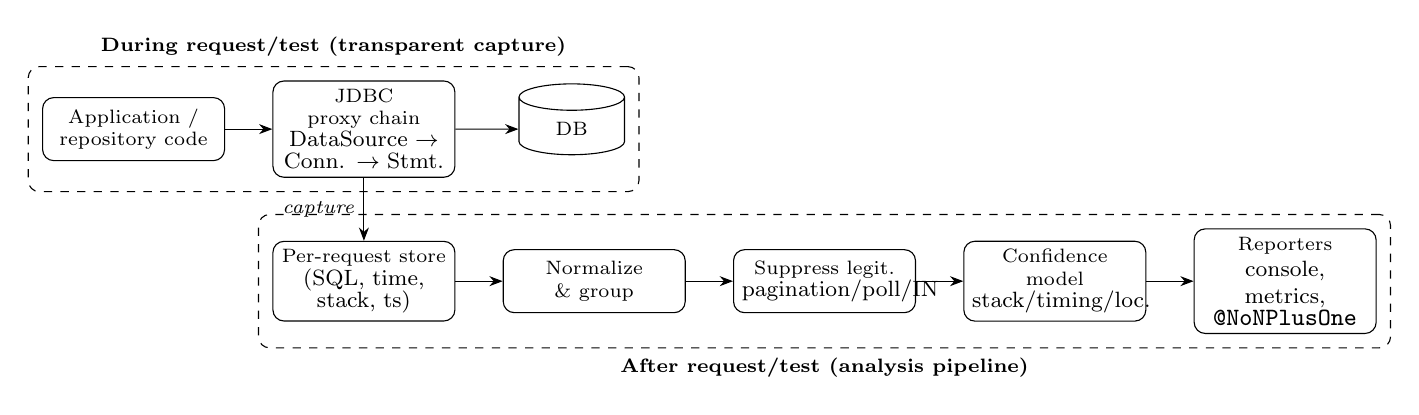
\begin{tikzpicture}[
  font=\scriptsize, >=Stealth, node distance=6mm,
  box/.style={draw, rounded corners, align=center, inner sep=3pt,
              minimum height=8mm, text width=2.1cm},
  db/.style={draw, cylinder, shape border rotate=90, aspect=0.25,
             align=center, inner sep=2pt, minimum height=9mm, text width=1.2cm},
  lbl/.style={midway, above, font=\scriptsize\itshape}
]
\node[box] (app) {Application / repository code};
\node[box, right=of app] (proxy) {JDBC proxy chain\\ \footnotesize DataSource $\to$ Conn. $\to$ Stmt.};
\node[db,  right=8mm of proxy] (dbms) {DB};
\node[box, below=8mm of proxy] (store) {Per-request store\\ \footnotesize(SQL, time, stack, ts)};
\node[box, right=of store] (norm) {Normalize\\ \& group};
\node[box, right=of norm] (supp) {Suppress legit.\\ \footnotesize pagination/poll/IN};
\node[box, right=of supp] (conf) {Confidence model\\ \footnotesize stack/timing/loc.};
\node[box, right=of conf] (rep) {Reporters\\ \footnotesize console, metrics,\\ \code{@NoNPlusOne}};

\draw[->] (app) -- (proxy);
\draw[->] (proxy) -- (dbms);
\draw[->] (proxy) -- node[left, font=\scriptsize\itshape]{capture} (store);
\draw[->] (store) -- (norm);
\draw[->] (norm) -- (supp);
\draw[->] (supp) -- (conf);
\draw[->] (conf) -- (rep);

\begin{scope}[on background layer]
  \node[draw, dashed, rounded corners, fit=(app)(proxy)(dbms),
        inner sep=5pt, label=above:{\scriptsize\bfseries During request/test (transparent capture)}] {};
  \node[draw, dashed, rounded corners, fit=(store)(norm)(supp)(conf)(rep),
        inner sep=5pt, label=below:{\scriptsize\bfseries After request/test (analysis pipeline)}] {};
\end{scope}
\end{tikzpicture}
\vspace{-3pt}
\caption{\tool{} architecture. A transparent JDBC proxy chain records every
statement into a per-request thread-local store; when the request (or test
method) ends, the analysis pipeline normalizes and groups statements, suppresses
legitimate repetition, scores remaining groups with the confidence model, and
routes issues to reporters.}
\Description{A two-phase pipeline: a capture phase wrapping the JDBC datasource,
connection, and statement, recording queries to a per-request store; and an
analysis phase that normalizes, suppresses legitimate repeats, scores with a
confidence model, and reports.}
\label{fig:arch}
\vspace{-8pt}
\end{figure*}

\tool{} (Fig.~\ref{fig:arch}) wraps the application's \code{DataSource} in a
chain of dynamic proxies (\code{DataSource}~$\to$ \code{Connection}~$\to$
\code{Statement}). Every executed statement is recorded (SQL text, execution
time, capturing call stack, and timestamp) into a per-request thread-local
store, giving complete request isolation with no locks. Request boundaries are
delimited by a servlet filter in production, or by the \code{@NoNPlusOne} JUnit~5
extension in tests. When the boundary closes, the analysis pipeline runs. The
tool ships as two artifacts: a dependency-free \emph{core} engine --- which also
provides the \code{@NoNPlusOne} annotation and JUnit~5 extension --- and a Spring
Boot \emph{starter} (auto-configuration, filter, Prometheus metrics, persistent
issue storage). Adoption requires one dependency and no code changes.



%% ===========================================================================
\section{Detection Approach}
%% ===========================================================================
\noindent\textbf{Normalization and grouping.} Captured SQL is normalized (string
and numeric literals are parameterized, comments stripped, whitespace
collapsed) while row-limiting clauses are preserved. Statements are then grouped
by normalized shape; only groups exceeding a minimum repetition count are
considered.

\noindent\textbf{False-positive suppression.} Before scoring, \tool{} discards
groups that match known-legitimate patterns: (i) \emph{pagination}, repeated
reads of one shape that all carry an \code{OFFSET} clause, including the common
case where the offset is a bind parameter (\code{OFFSET ? ROWS FETCH ...}) and no
literal is visible; (ii) \emph{streaming/polling}, a timestamp predicate read at
a steady cadence; (iii) \emph{batched} \code{IN (...)} fetches; and (iv)
sub-threshold repetition. Crucially, a bare repeated \code{LIMIT n} with no offset
is \emph{not} treated as pagination, since it can be a genuine row-limited N+1.

\begin{figure}[t]
\centering
\begin{tikzpicture}[
  font=\scriptsize, >=Stealth,
  sig/.style={draw, rounded corners, align=center, inner sep=2pt,
              minimum height=6mm, text width=2.0cm, fill=gray!5},
  sum/.style={draw, circle, inner sep=0.5pt, minimum size=6mm, fill=gray!10},
  dec/.style={draw, diamond, aspect=1.5, inner sep=0pt, align=center,
              minimum width=11mm, fill=gray!5},
  out/.style={draw, rounded corners, align=center, inner sep=2.5pt,
              minimum height=4.5mm, minimum width=11mm}
]
\node[sig] (sf) {Framework $S_f$\\[-1pt]\tiny ORM/lazy-load frames};
\node[sig, below=2.0mm of sf] (st) {Timing $S_t$\\[-1pt]\tiny loop tightness};
\node[sig, below=2.0mm of st] (sl) {Location $S_l$\\[-1pt]\tiny call-site proximity};
\node[sum, right=9mm of st] (sum) {$\Sigma$};
\node[dec, right=8mm of sum] (dec) {$S\!\ge\!\theta$};
\node[out, right=7mm of dec, yshift=4.5mm, fill=black!78, text=white] (flag) {N+1};
\node[out, right=7mm of dec, yshift=-4.5mm] (pass) {legit.};
\draw[->] (sf.east) -- node[above,sloped,font=\tiny]{$w_f{=}.5$} (sum);
\draw[->] (st.east) -- node[above,font=\tiny,pos=.55]{$.2$} (sum);
\draw[->] (sl.east) -- node[below,sloped,font=\tiny]{$w_l{=}.3$} (sum);
\draw[->] (sum) -- node[above,font=\tiny]{$S$} (dec);
\draw[->] (dec.east) |- node[above,font=\tiny,pos=.75]{yes} (flag.west);
\draw[->] (dec.east) |- node[below,font=\tiny,pos=.75]{no} (pass.west);
\end{tikzpicture}
\vspace{-3pt}
\caption{Confidence model. Each group that survives suppression is scored by three
bounded signals, fused into $S\in[0,1]$ by fixed weights, and compared to a decision
threshold $\theta$. Signal diversity is deliberate: no single signal decides alone, so a
strong loop with weak framework evidence (or vice versa) is still scored on its merits.}
\label{fig:confidence}
\vspace{-10pt}
\end{figure}

\noindent\textbf{Confidence model.} Surviving groups are scored with a confidence metric $S \in [0, 1]$ (Fig.~\ref{fig:confidence}), computed as a weighted sum of three normalized signals:
\begin{equation}
  S = w_f \cdot S_f + w_t \cdot S_t + w_l \cdot S_l
\end{equation}
where $w_f$, $w_t$, and $w_l$ represent weights for the \emph{framework}, \emph{timing}, and \emph{location} signals respectively, satisfying $w_f + w_t + w_l = 1.0$ (by default, $w_f=0.5, w_t=0.2, w_l=0.3$).
The signals are defined as follows:
\begin{itemize}[leftmargin=*,topsep=1pt,itemsep=1pt]
  \item \textbf{Framework ($S_f$)} scores the likelihood of ORM involvement from the strongest stack-trace evidence in the group, scaled by how many of the group's queries exhibit it. Definite collection lazy loading (e.g., Hibernate \code{PersistentBag}) is the top tier, scoring $S_f \in [0.7, 1.0]$ --- $1.0$ when it dominates the group, never below $0.7$ when present; ORM or repository entry-points (e.g., Spring \code{SimpleJpaRepository}) form a middle tier scoring $S_f \in [0.3, 0.7]$; and bare JDBC/connection-pool frames score $S_f = 0.0$, so the model is not biased by driver infrastructure present in every query. This signal is therefore ORM-aware: on non-ORM (plain JDBC) stacks it stays silent and detection leans on the timing and location signals, which RQ1 confirms still suffices.
  \item \textbf{Timing ($S_t$)} uses the group's combined query execution time as a proxy for loop tightness, since queries fired in a tight loop complete in a short aggregate burst: $S_t = 1.0$ when the total is under $1\text{\,s}$, $S_t = 0.7$ when under $3\text{\,s}$, and $S_t = 0.3$ otherwise. Groups whose queries arrive at a steady cadence are first classified as deliberate pacing and handled by suppression rather than scored as loops.
  \item \textbf{Location ($S_l$)} measures the structural proximity of query origins: $S_l = 1.0$ if all queries stem from the exact same file and line; $S_l = 0.9$ if they share a method; $S_l = 0.8$ if they share a class; $S_l = 0.7$ if a deep loop structure is inferred via a shared ancestor call frame with differing iteration sites; and $S_l = 0.5$ for unrelated scattered origins.
\end{itemize}
These per-signal values and weights are pragmatic, hand-set defaults rather than learned parameters; Section~\ref{sec:eval} shows the resulting verdicts are robust to the precise weights and decision threshold. Three modes are supported: \textsc{Threshold} (count only), \textsc{Confidence} (score only), and \textsc{Hybrid} (both must agree). Section~\ref{sec:eval} shows what the model adds over a pure threshold.

\noindent\textbf{Plans and fixes.} For severe issues, \tool{} can run
\texttt{EXPLAIN} (MySQL, PostgreSQL, H2) to flag full scans and missing indexes.
Each report includes a framework-specific suggestion: \code{JOIN FETCH},
\code{@EntityGraph}, or \code{@BatchSize} for Hibernate; nested result maps for
MyBatis; \code{multiset()}/joins for jOOQ; \code{IN}-batching for Spring JDBC.

%% ===========================================================================
\section{Using Query Analyzer}
%% ===========================================================================
\noindent\textbf{Production.} Adding the starter dependency is enough; on the next
request \tool{} reports, per endpoint, the offending table, a sample query, a
confidence-scored explanation, and a fix:
\begin{lstlisting}[language={}]
N+1 Query Detected
  Endpoint   GET /owners
  Location   OwnerController.findPaginated...:130
  Problem    5 repeated queries for 'pets'
  Suggestions  Confidence: HIGH (100%)
    ORM lazy loading in stack; tight loop; same site
\end{lstlisting}

\noindent\textbf{Tests (shift-left).} The \code{@NoNPlusOne} annotation turns
detection into a regression guard that fails the build on reintroduction:
\begin{lstlisting}
@Test @NoNPlusOne
void listing_isNotNPlusOne() {
    service.findAllWithOrders();   // fails if an N+1 occurs
}
\end{lstlisting}
A profile (\textsc{Strict}/\textsc{Balanced}/\textsc{Lenient}), the detection
mode, and per-table ignores are configurable; defaults work out of the box.

%% ===========================================================================
\section{Evaluation}
\label{sec:eval}
%% ===========================================================================
We answer four questions. \textbf{RQ1:} how accurate is \tool{} versus a
count-based baseline? \textbf{RQ2:} does the confidence model add value over a
simple threshold? \textbf{RQ3:} does it find real defects in unmodified code, and
are its fixes effective? \textbf{RQ4:} what is its overhead? All experiments ship
in a \code{query-analyzer-benchmark} module and run with one command; numbers
below are from a commodity laptop. The controlled benchmark runs on H2,
Hibernate~6.3, and Spring~Boot~3.2; the PetClinic case study (RQ3) uses
PetClinic's last Spring~Boot~3 revision (commit \code{66747e3}).

\noindent\textbf{Setup.} A labelled suite of seven JPA workloads is executed
against a real database; each query trace is captured once and replayed,
unchanged, to every detector, so the only variable is the algorithm. We compare
against three baselines: a faithful re-implementation of the count-based rule
used by test tools; the \emph{real} Hypersistence Utils binary; and the
\emph{real} JPlusOne binary (jplusone-core~2.0.0) --- a modern automatic N+1
detector --- both run live on the same Spring~Boot~3 / Hibernate~6 stack with
their verdicts read from their own output. JPlusOne is the only other test-time
N+1 detector ported to the Jakarta/Hibernate~6 stack: spring-hibernate-query-utils
and QuickPerf both remain on Spring~Boot~2 / Hibernate~5 (\code{javax}) and do not
load on a modern application --- itself a symptom of the fragmentation \tool{}
addresses.

\noindent\textbf{Feature comparison.} Table~\ref{tab:features} situates \tool{}
against representative tools. It is the only free tool that is simultaneously
framework-agnostic, usable in test \emph{and} production, false-positive-aware,
and plan-aware.

\begin{table}[t]
\centering
\caption{Capability comparison (\cmark\ yes, \pmark\ partial, \xmark\ no).
P6Spy/datasource-proxy are interceptors, not detectors.}
\label{tab:features}
\scriptsize
\setlength{\tabcolsep}{3.2pt}
\renewcommand{\arraystretch}{1.1}
\begin{tabular}{l cccc >{\columncolor{gray!14}}c}
\toprule
Capability & \rotatebox{60}{P6Spy/dsp} & \rotatebox{60}{QuickPerf} & \rotatebox{60}{JPlusOne} & \rotatebox{60}{Hyp.\,Utils} & \rotatebox{60}{\textbf{\tool}} \\
\midrule
Framework-agnostic (JDBC)      & \cmark & \pmark & \xmark & \xmark & \cmark \\
Detects N+1 automatically      & \xmark & \cmark & \cmark & \pmark & \cmark \\
\addlinespace[2.5pt]
Test-time use                  & \pmark & \cmark & \cmark & \cmark & \cmark \\
Production runtime use         & \cmark & \xmark & \pmark & \xmark & \cmark \\
\addlinespace[2.5pt]
False-positive suppression     & \xmark & \xmark & \xmark & \xmark & \cmark \\
Confidence scoring             & \xmark & \xmark & \xmark & \xmark & \cmark \\
Query-plan (\texttt{EXPLAIN})  & \xmark & \xmark & \xmark & \xmark & \cmark \\
Fix suggestions                & \xmark & \pmark & \xmark & \xmark & \cmark \\
\addlinespace[2.5pt]
Open source                    & \cmark & \cmark & \cmark & \cmark & \cmark \\
\bottomrule
\end{tabular}
\vspace{-4pt}
\end{table}

\noindent\textbf{RQ1 (accuracy).} Table~\ref{tab:accuracy} reports precision,
recall, and F1 on the seven-scenario suite (2 true N+1, 5 clean; this small,
hand-built suite validates the mechanism rather than estimating field accuracy,
see Limitations). \tool{} flags both N+1s and none of the five clean cases
(2~TP, 0~FP, 5~TN, 0~FN); the count-based baseline catches both N+1s but also
fires on three of the five clean scenarios---pagination, polling, and
sub-threshold repetition---for 0.40 precision. JPlusOne, run live, is precise
(1.00) and correctly flags the lazy-collection N+1, but its model, by design,
tracks only Hibernate lazy initialisations: it does not recognise an N+1
expressed as a repository query-method invoked once per row, missing that case
(0.50 recall, 0.67~F1), and it has no production mode. The live Hypersistence counter returns raw statement
counts (e.g.\ 6 for an N+1, 5 for legitimate pagination): a count alone cannot
separate the two without a human-specified expected value, and it runs only in
tests. \tool{} detects both N+1 forms and suppresses all legitimate repetition.
To check that detection is not Hibernate-bound, we also ran an N+1 written in
\emph{plain JDBC} with no ORM (raw \code{PreparedStatement}, so the framework
signal scores zero): all three modes still detect it, confirming the
JDBC-layer design generalises beyond ORM stacks.

\begin{table}[t]
\centering
\caption{Detection accuracy on the labelled suite (7 scenarios; 2 true N+1, 5
clean). JPlusOne and the count-based baseline are run live on the same stack;
per-scenario verdicts and raw confusion counts are in the artifact.}
\label{tab:accuracy}
\small
\begin{tabular}{lccc}
\toprule
Detector & Precision & Recall & F1 \\
\midrule
\tool{} (Threshold/Confidence/Hybrid) & \textbf{1.00} & \textbf{1.00} & \textbf{1.00} \\
JPlusOne 2.0.0 (live)                  & 1.00 & 0.50 & 0.67 \\
Count-based baseline (QuickPerf-style) & 0.40 & 1.00 & 0.57 \\
\bottomrule
\end{tabular}
\vspace{-4pt}
\end{table}

\noindent\textbf{RQ2 (model contribution).} On the suite above, \textsc{Threshold}
and \textsc{Confidence} tie, because suppression alone handles those cases. To
isolate the model we use a controlled study with one extra case class,
\emph{scattered repeats} (the same query from several call sites in one request).
Here a pure threshold false-positives (precision 0.60) while
\textsc{Confidence}/\textsc{Hybrid} reach 1.00. An ablation
(Table~\ref{tab:ablation}) shows each signal earns its place: removing the
framework signal costs precision; removing timing or location costs recall.
Sweeping the decision threshold $\theta$ (Fig.~\ref{fig:sensitivity}), F1 peaks across $0.4$--$0.5$, justifying the choice of $\theta=0.5$. The weights are not a knife-edge: sweeping every $(w_f,w_t,w_l)$ on a $0.1$ grid (each in $[0.1,0.8]$, summing to~1) keeps F1 in $[0.75,1.00]$, its worst case never falling below the threshold baseline, and a broad region including the default $(0.5,0.2,0.3)$ reaches the optimal F1${=}1.00$ (10 of 36 grid points). The ordering reflects signal reliability: the framework signal most directly evidences ORM lazy loading and is weighted highest, timing (the noisiest) lowest.

\begin{figure}[t]
\centering
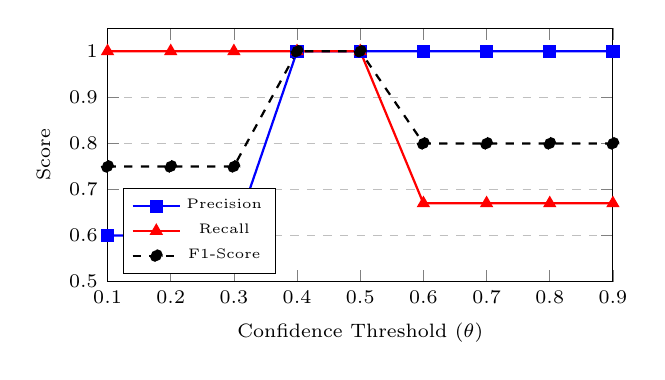
\begin{tikzpicture}
\begin{axis}[
    xlabel={Confidence Threshold ($\theta$)},
    ylabel={Score},
    xmin=0.1, xmax=0.9,
    ymin=0.5, ymax=1.05,
    xtick={0.1,0.2,0.3,0.4,0.5,0.6,0.7,0.8,0.9},
    ytick={0.5,0.6,0.7,0.8,0.9,1.0},
    legend pos=south west,
    ymajorgrids=true,
    grid style=dashed,
    height=4.8cm,
    width=8.0cm,
    tick label style={font=\scriptsize},
    label style={font=\scriptsize},
    legend style={font=\tiny}
]
\addplot[
    color=blue,
    mark=square*,
    thick
]
    coordinates {
    (0.1,0.60)(0.2,0.60)(0.3,0.60)(0.4,1.00)(0.5,1.00)(0.6,1.00)(0.7,1.00)(0.8,1.00)(0.9,1.00)
    };
\addlegendentry{Precision}

\addplot[
    color=red,
    mark=triangle*,
    thick
]
    coordinates {
    (0.1,1.00)(0.2,1.00)(0.3,1.00)(0.4,1.00)(0.5,1.00)(0.6,0.67)(0.7,0.67)(0.8,0.67)(0.9,0.67)
    };
\addlegendentry{Recall}

\addplot[
    color=black,
    mark=*,
    thick,
    dashed
]
    coordinates {
    (0.1,0.75)(0.2,0.75)(0.3,0.75)(0.4,1.00)(0.5,1.00)(0.6,0.80)(0.7,0.80)(0.8,0.80)(0.9,0.80)
    };
\addlegendentry{F1-Score}
\end{axis}
\end{tikzpicture}
\vspace{-6pt}
\caption{Sensitivity analysis sweeping the confidence threshold $\theta$. F1-score peaks at $[0.4, 0.5]$, justifying the choice of $\theta=0.5$.}
\label{fig:sensitivity}
\vspace{-10pt}
\end{figure}

\begin{table}[t]
\centering
\caption{Controlled study: confidence-model contribution and ablation
(weights renormalized when a signal is removed).}
\label{tab:ablation}
\small
\begin{tabular}{lccc}
\toprule
Configuration & Precision & Recall & F1 \\
\midrule
\textsc{Threshold} (count only) & 0.60 & 1.00 & 0.75 \\
\textsc{Confidence} / \textsc{Hybrid} & \textbf{1.00} & \textbf{1.00} & \textbf{1.00} \\
\midrule
Full model & 1.00 & 1.00 & 1.00 \\
\quad -- no framework signal & 0.60 & 1.00 & 0.75 \\
\quad -- no timing signal    & 1.00 & 0.67 & 0.80 \\
\quad -- no location signal  & 1.00 & 0.67 & 0.80 \\
\bottomrule
\end{tabular}
\vspace{-6pt}
\end{table}

\noindent\textbf{RQ3 (real-world).} We added \tool{} to the unmodified Spring
PetClinic~\cite{petclinic} (one dependency, zero code changes) and exercised its
pages, including the paginated \code{/owners} listing. It detected three real
N+1s, all at high (100\%) confidence, each located to a stack frame:
\code{vet\_specialties} (5 queries), \code{pets} (5), and \code{visits} (6), the
last two traced to \code{OwnerController:130} (the pagination handler). Across these
pages it reported only these three genuine N+1s and raised no false positives on
the single-shot pagination and reference-data queries issued by the same
requests. Applying the tool's own suggested fix
(\code{@BatchSize}) and re-running eliminated all three (3~$\to$~0), confirming the
suggestions are not merely diagnostic but actionable. As further corroboration on
unrelated code, applying \tool{} (one dependency, no code changes) to a
third-party Spring~Boot~3 many-to-many sample flagged a \emph{serialization-time}
N+1 --- five repeated tag loads on \code{GET /api/tutorials} at 100\% confidence
--- a different manifestation from PetClinic's controller-loop N+1.

\noindent\textbf{RQ4 (overhead).} Measured live against a real PostgreSQL
instance on a laptop (Intel Core i7-9750H, 6~cores, 16\,GB RAM), \tool{} adds a
fixed per-request overhead on the order of $1$\,ms for a six-query trace
($\approx\!0.7$\,ms in our runs: statement capture plus post-request analysis,
with the exact figure and the split between the two varying with hardware). Because this
cost is per-request, not proportional to query latency, it stays below 5\% for
any request taking $\gtrsim\!20$\,ms and below 2\% at 50\,ms --- negligible for
realistic DB-backed endpoints, and dominating only on sub-millisecond in-memory
queries. On the same instance the tool's \texttt{EXPLAIN} analyzer correctly
classified the N+1 child query as a sequential scan (\code{cost=0.00..11.62}) and
recommended an index.

\noindent\textbf{Limitations.} \tool{} records queries in a per-request
thread-local store, so it assumes a request is served on a single thread:
reactive/asynchronous stacks (e.g.\ Spring WebFlux), where one request hops
threads, are not yet supported. Detection is single-JVM --- an N+1 caused by a
downstream microservice is invisible. The labelled suite is small and its
scenarios align with the suppression categories, so it validates the mechanism
rather than establishing field accuracy; the generalisation evidence is the
unmodified-PetClinic study and the plain-JDBC case, not the synthetic suite. The
real-world study covers one application on one ORM, though the plain-JDBC result
shows the JDBC-level design is not ORM-bound. Production overhead is
characterised (RQ4) but not measured under sustained load; the reported cost is a
fixed per-request figure, not a percentage guarantee. All artifacts are public
for scrutiny and replication.

%% ===========================================================================
\section{Related Work}
%% ===========================================================================
Academic work establishes that ORM/database anti-patterns are common and
impactful and proposes detection or repair, often statically or for specific
stacks (e.g.\ Rails)~\cite{chen2014orm, yang2018webapps, yang2019powerstation}.
\tool{} is complementary: a dynamic, framework-agnostic, deploy-and-test tool for
the JVM. Among practitioner tools, P6Spy~\cite{p6spy} and
datasource-proxy~\cite{datasourceproxy} provide interception but no detection;
QuickPerf~\cite{quickperf}, JPlusOne~\cite{jplusone},
spring-hibernate-query-utils~\cite{springhibernatequeryutils}, and Hypersistence
Utils~\cite{hypersistenceutils} detect N+1 but are test-only and mostly
Hibernate-specific, and, as Table~\ref{tab:features} and our experiments
show, lack false-positive suppression and confidence scoring.
Table~\ref{tab:accuracy} quantifies the resulting precision gap.

%% ===========================================================================
\section{Conclusion}
%% ===========================================================================
\tool{} brings framework-agnostic, confidence-based N+1 and slow-query detection
to the JVM, usable both as a CI regression guard and in production, with
actionable fixes. It is released under MIT on Maven Central
(\code{io.github.query-analyzer}, v1.2.5); source, the benchmark module, and the
Spring PetClinic case study are at
\url{https://github.com/query-analyzer/query-analyzer}. Step-by-step
reproduction instructions for every experiment accompany the artifact.

\clearpage
\bibliographystyle{ACM-Reference-Format}
\bibliography{refs}

\end{document}
